\documentclass[a4paper,12pt]{article}
\usepackage{ctex}
\usepackage{geometry}
\usepackage{amsmath}
\usepackage{amssymb}
\usepackage{amsthm}
\usepackage{graphicx}
\usepackage{listings}
\usepackage[colorlinks=true, linkcolor=blue]{hyperref}
\usepackage{booktabs}
\usepackage{float}
\usepackage{color}
\usepackage{subfigure}


\geometry{left=2cm, right=2cm, top=2cm, bottom=2cm}

% 用来设置附录中代码的样式

\lstset{
    basicstyle          =   \sffamily,          % 基本代码风格
    keywordstyle        =   \bfseries,          % 关键字风格
    commentstyle        =   \rmfamily\itshape,  % 注释的风格,斜体
    stringstyle         =   \ttfamily,  % 字符串风格
    flexiblecolumns,                % 别问为什么,加上这个
    numbers             =   left,   % 行号的位置在左边
    showspaces          =   false,  % 是否显示空格,显示了有点乱,所以不现实了
    numberstyle         =   \zihao{-5}\ttfamily,    % 行号的样式,小五号,tt等宽字体
    showstringspaces    =   false,
    captionpos          =   t,      % 这段代码的名字所呈现的位置,t指的是top上面
    frame               =   lrtb,   % 显示边框
}

\lstdefinestyle{Verilog}{
    language        =   Verilog, % 语言选Python
    basicstyle      =   \zihao{-5}\ttfamily,
    numberstyle     =   \zihao{-5}\ttfamily,
    keywordstyle    =   \color{blue},
    keywordstyle    =   [2] \color{teal},
    stringstyle     =   \color{magenta},
    commentstyle    =   \color{red}\ttfamily,
    breaklines      =   true,   % 自动换行,建议不要写太长的行
    columns         =   fixed,  % 如果不加这一句,字间距就不固定,很丑,必须加
    basewidth       =   0.5em,
}


\title{ICE2603 课程大作业实验报告}
\author{521030910117 朱鹏翔\footnote{感谢陈颖琪老师和几位助教一个学期的辛勤付出}}

\begin{document}
    \maketitle

    \section{实验简介}

    本次实验主要分为两部分,主要在Lab 4的代码基础上进行扩展,分别为程序执行周期数的采样模块设计与实现以及基于已有的22条指令的极值搜索程序的设计仿真和板级验证。在这两次实验中,要求对I/O接口进行熟练应用,并培养自行设计新模块以实现特定功能的能力。同时,也对RISC-V的掌握程度做了更进一步的要求,需要自行完成汇编语言的设计与其在CPU上的一系列操作,以得到正确的结果,是对本学期实验课程的总结。

    \section{实验器材}

    Xilinx 的Vivado 开发套件(2020.2 版本),Xilinx 的EGO1 FPGA开发板。本次实验为综合性设计,需要虚拟仿真以及对应的板级验证。

    \section{实验一分析}

    首先,我们在Lab 4代码的基础上在I/O接口处添加\verb|in_port2|用于时钟周期计数的输入。为此,我们需要修改Inport模块的底层设计。在\verb|io_input|模块中,我们将地址\verb|0x88|作为\verb|in_port2|的对应地址,一旦\verb|lw|指令从\verb|0x88|中取数,那么将返回\verb|in_port2|的值。具体实现如下所示

    \begin{lstlisting}[language=verilog]
module io_input_mux(
    input [31:0] a0,
    input [31:0] a1,
    input [31:0] a2,
    input [5:0] sel_addr,
    output reg [31:0] y
);

    always @* begin
        case (sel_addr)
            6'b100000: y = a0;  // in_port0 byte address 0x80
            6'b100001: y = a1;  // in_port1 byte address 0x84
            6'b100010: y = a2;  // in_port2 byte address 0x88
            default: y = 32'h0;
        endcase
    end
endmodule
    \end{lstlisting}

    之后,我们设计了一个具有异步清零功能的32bit计数器\verb|sys_clk_counter|,对FPGA板上100MHz的输入系统时钟\verb|sys_clk_in|计数,同时设置板上\verb|sys_rst_n|按键可异步清零。其实现可如下所示,注意在这里需要采用时序逻辑进行处理,在上升沿触发。

\begin{lstlisting}[language=verilog]
module sys_clk_counter(
    input sys_clk_in, //100MHz clock
    input sys_rst_n,  //active low asynchronous reset
    output reg [31:0] count //32-bit counter output
);

//increment counter on positive edge of sys_clk_in
always @(posedge sys_clk_in) begin
    if (sys_rst_n == 1'b0) //asynchronous reset
        count <= 32'b0;
    else
        count <= count + 1;
end

endmodule
\end{lstlisting}
    
    之后添加计数器到顶层模块\verb|sc_cpu_iotest|,计数器输出连接到\verb|in_port2|,其代码实现如下所示。注意这里并不再需要进行扩展,直接将\verb|count|变量赋值给\verb|in_port2|即可。
\begin{lstlisting}[language=verilog]
// added for final project. generate sys_clk_counter
sys_clk_counter clk_counter(sys_clk_in, sys_rst_n, count);

// assign in_port2 to be the value of count
assign in_port2[31:0] = count;
\end{lstlisting}

    为了验证\verb|in_port2|以及时钟周期执行的正确性,我们再进一步进行如下操作。在测试程序执行结束时,也即在语句\verb|srli x18, x18, 15|和\verb|fi:j fi|之间添加程序段,旨在通过\verb|in_port2|读入计数器\verb|sys_clk_counter|的值,存于\verb|x20|,并通过\verb|outport2|(地址也是\verb|0x88|)输出到FPGA板七段数码管上。该值代表了程序执行到读计数器值语句所用的周期数的两倍。具体而言,我们所添加的RISC-V汇编代码如下所示。我们首先赋值\verb|x21=0x88|,\verb|x22=0x84|,之后利用\verb|sw|与输出端口,\verb|lw|与输入端口之间的联系便可以实现数据与I/O端口的交互功能。

    \begin{lstlisting}
addi x21, x0, 136
addi x22, x0, 132
lw x20, 0(x21)
sw x20, 0(x21)
sw x18, 0(x22)
    \end{lstlisting}

    \textbf{需要特别注意的是,由于以上代码的加入,会导致其它部分的某些跳转指令的PC值的改变,也即机器码的改变}。为此,在进行\verb|.coe|文件的更新时,需要将上述代码与原始测试代码进行整合后重新得到机器码,逐行验证并更新。最后,我们调整数码管端口的设定,如下所示。我们加入\verb|dec76|以在最高位显示学号的最后两位\verb|17|,并在中间两位加入\verb|pc|的值以便于后续结果的验证。

    \begin{lstlisting}[language=verilog]
// out_port_hex2dec unit, outport the first few numbers of the student number
out_port_hex2dec dec76(student_id, HEX4b7, HEX4b6);

//display unit, seven segment decode and digitron drive 
display display(
    .clk(sys_clk_in),
    .reset(sys_rst_n),
    .s({HEX4b7, HEX4b6, pc[7:0], HEX4b3, HEX4b2, HEX4b1, HEX4b0}),
    .seg0(seg_data_0_pin),
    .seg1(seg_data_1_pin),
    .ans(seg_cs_pin)
);
    \end{lstlisting}
    
    
    在完成了上述设置之后,我们对代码进行仿真,得到的结果如图\ref{fig:lab1_sim}所示。从仿真结果中我们可以看出,代码在执行至\verb|sw x20, 0(x21)|时于\verb|out_port2|输出当前的时钟周期数;而在运行指令\verb|sw x18, 0(x22)|后输出寄存器\verb|x18|当前的值。因而此时显示的时钟周期为\verb|CYC 152|,实际为\verb|CYC 76|。更进一步地,我们将上述猜想在Ripes仿真平台上进行验证,结果如图\ref{fig:lab1_ripes}所示,符合预期。最后,我们进行了板级验证,呈现的结果如图\ref{fig:lab1_board}所示,与仿真结果与Ripes验证的结果均匹配。这样,也就基本完成了实验一的相关设计。对于板级验证更加细致的介绍,可见提交的演示视频。

    \begin{figure}[htbp]
        \centering
        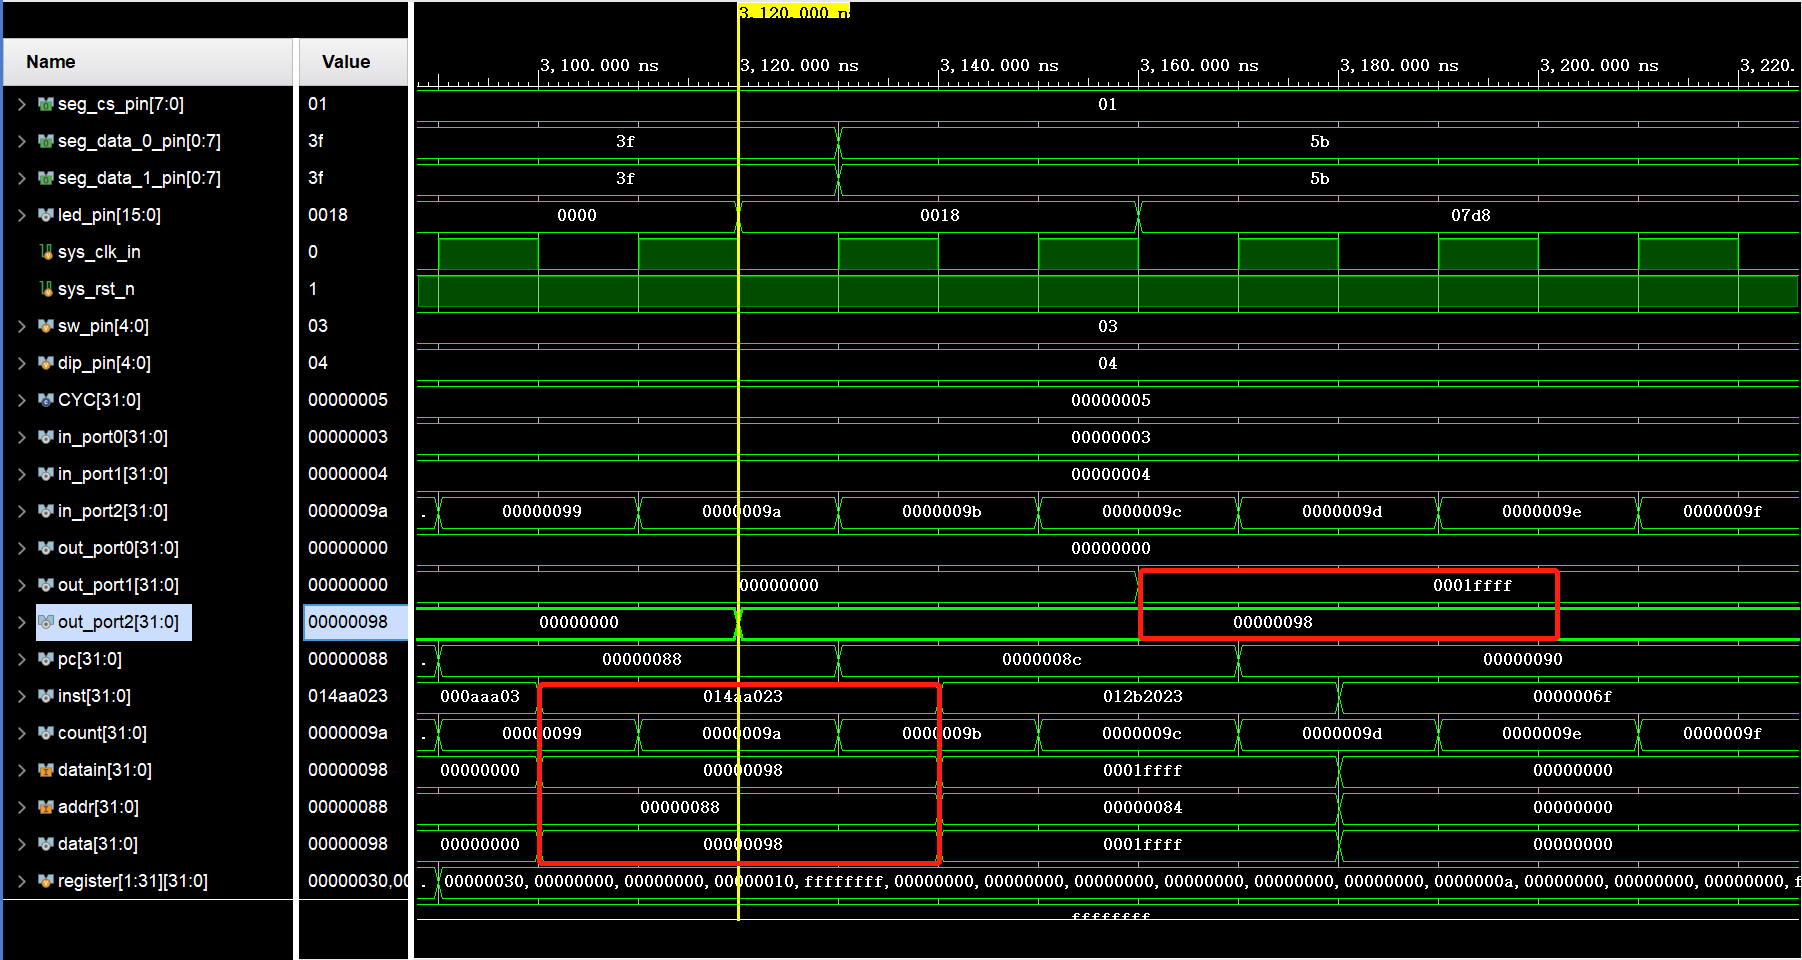
\includegraphics[scale=0.5]{fig2.png}
        \caption{实验一仿真结果分析}
        \label{fig:lab1_sim}
    \end{figure}
    
    \begin{figure}[htbp]
        \centering
        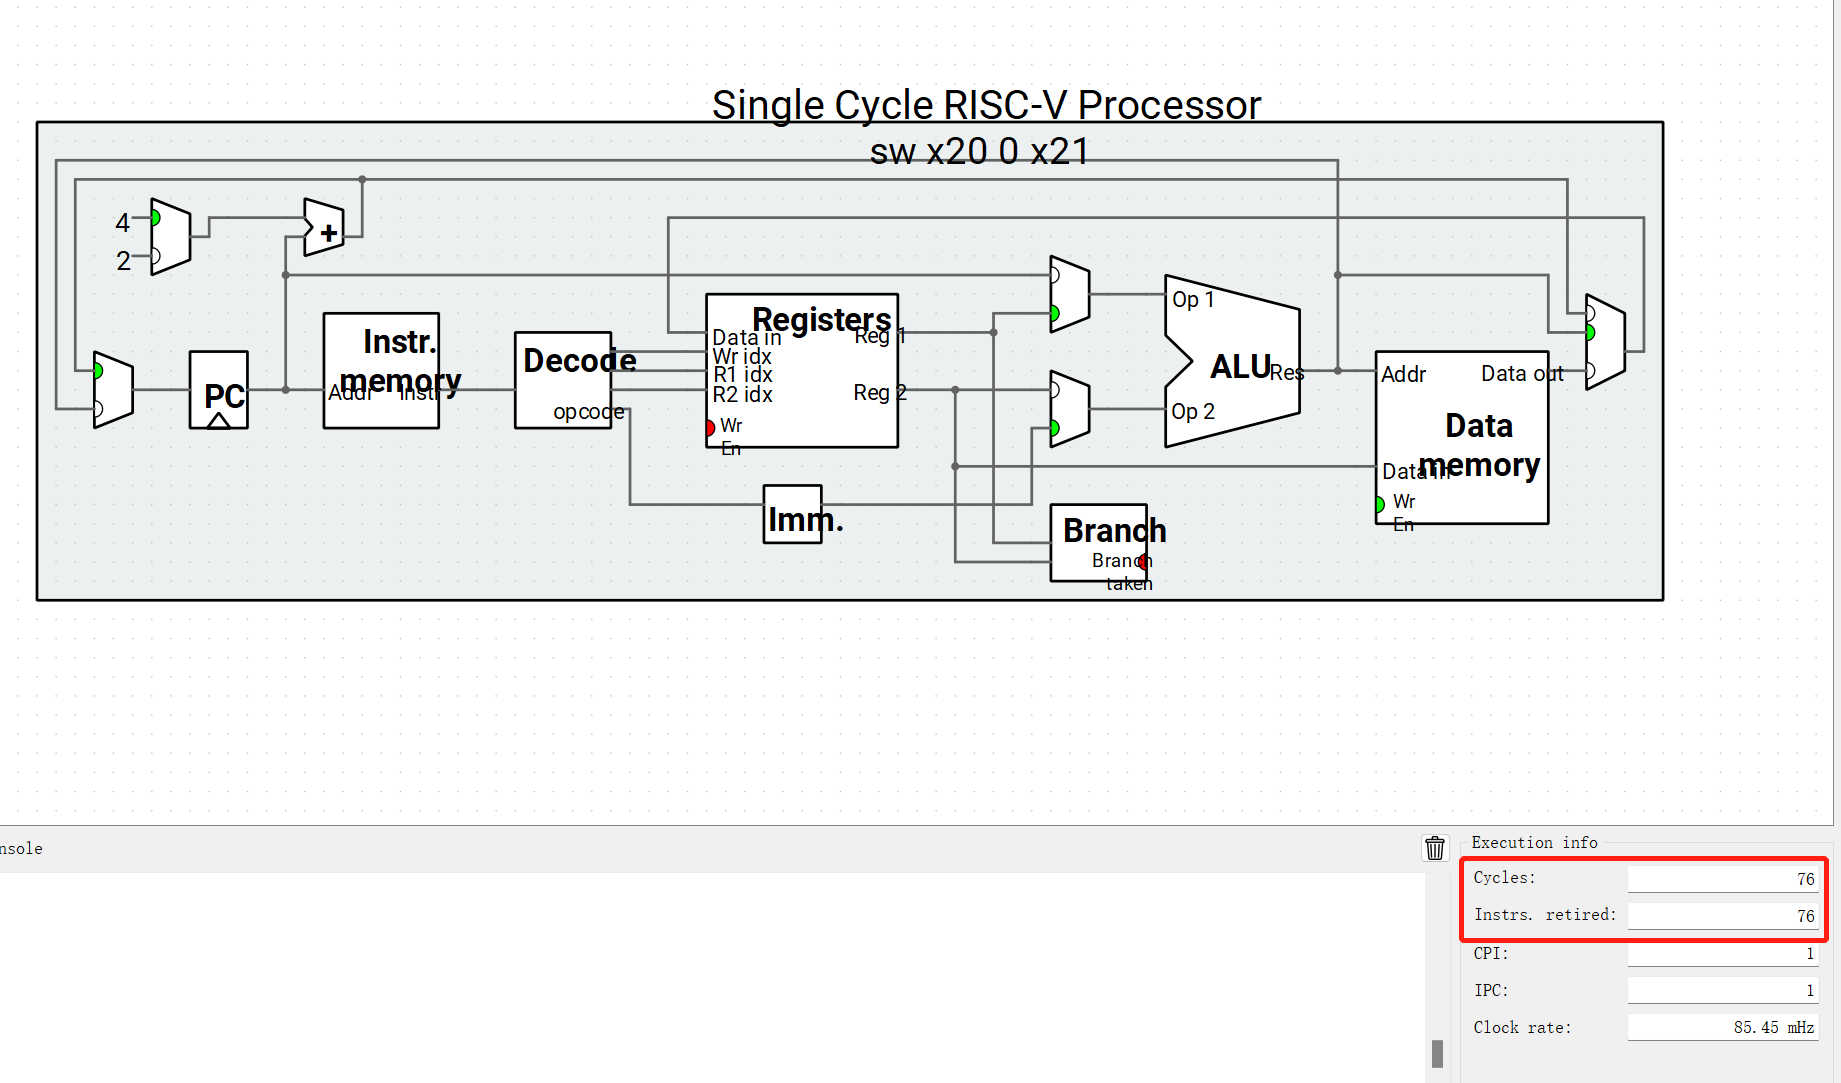
\includegraphics[scale=0.4]{fig3.png}
        \caption{实验一Ripes结果验证}
        \label{fig:lab1_ripes}
    \end{figure}

    \begin{figure}[htbp]
        \centering
        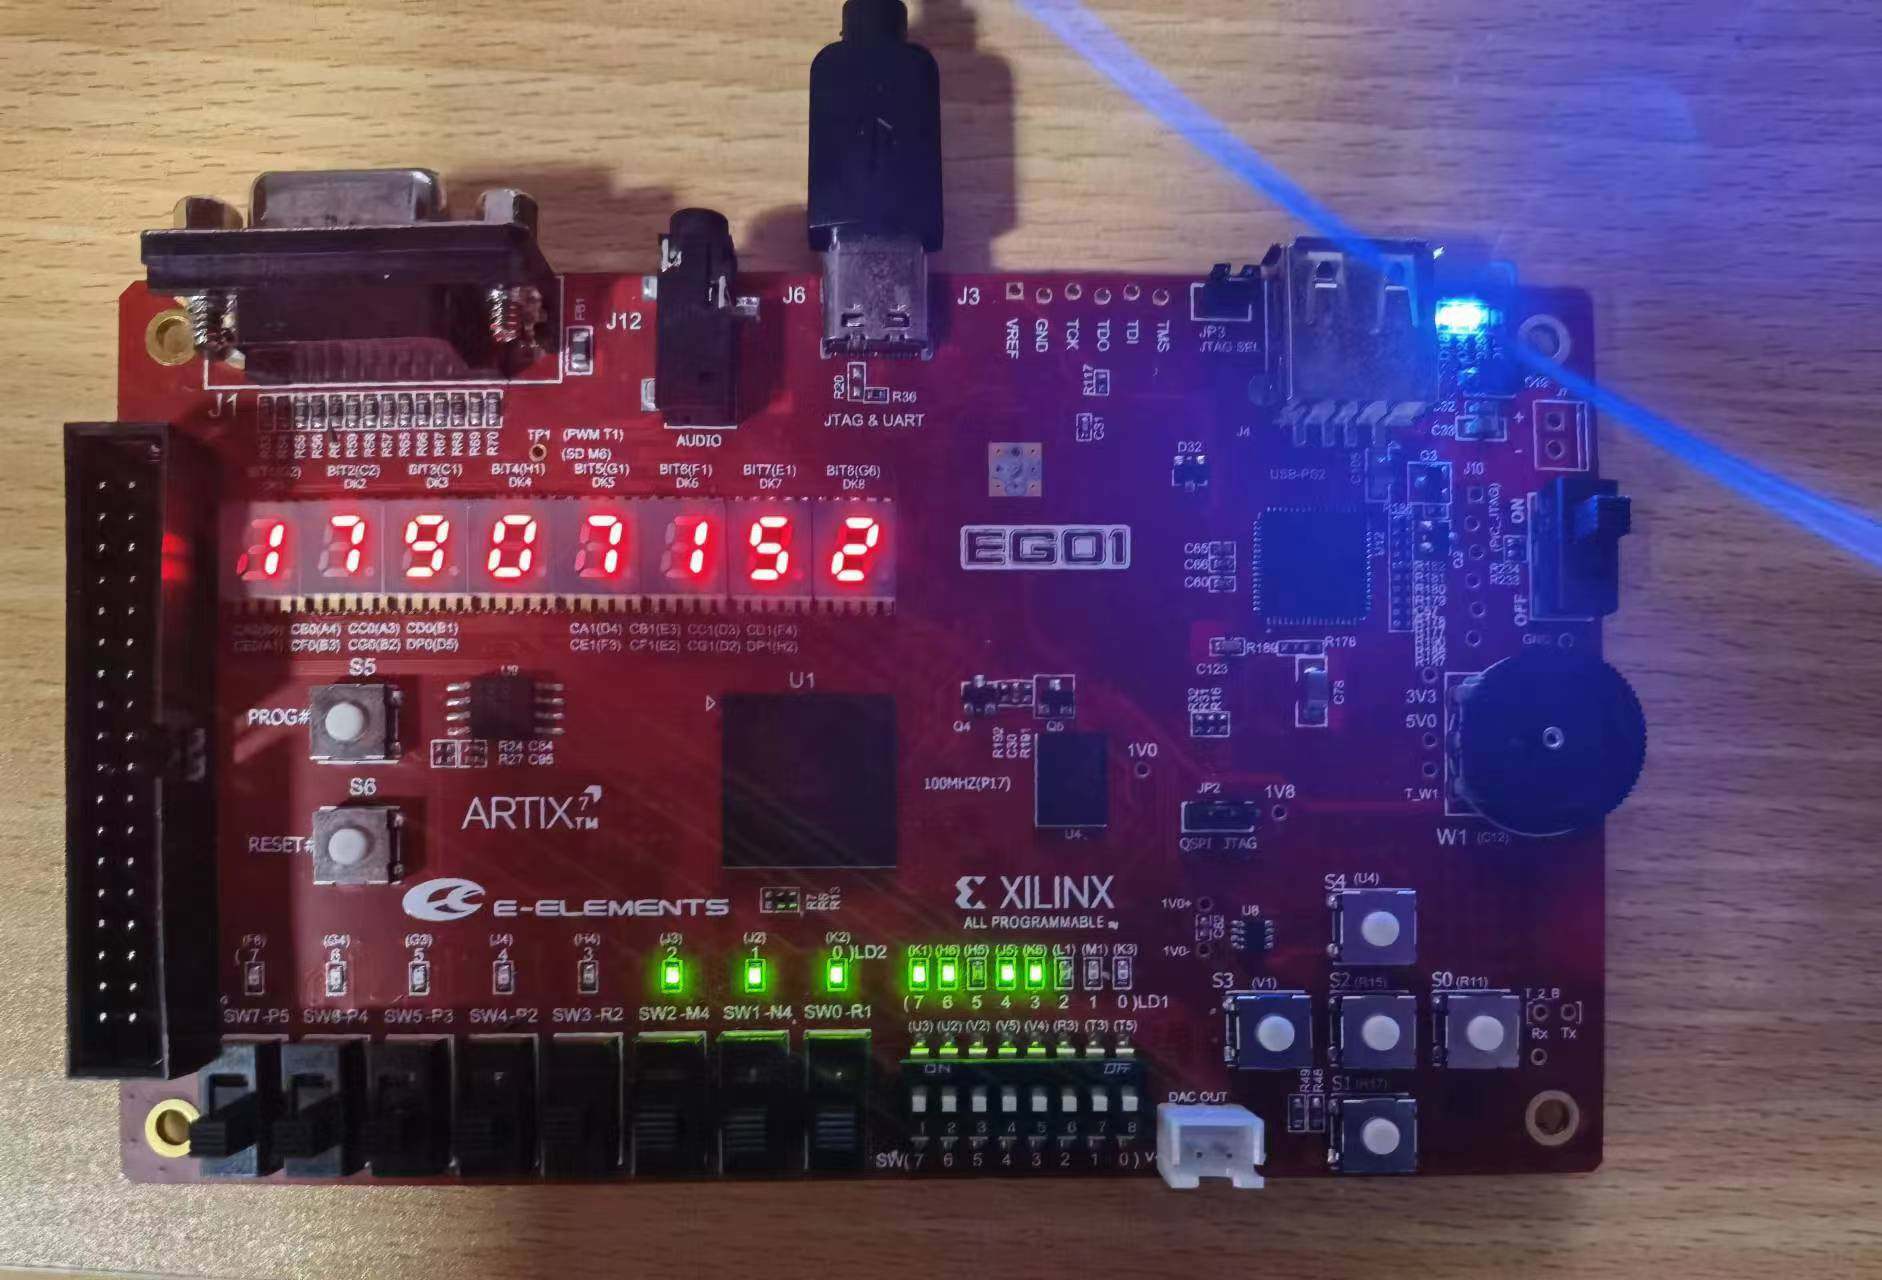
\includegraphics[scale=0.15]{fig1.jpg}
        \caption{实验一板级验证}
        \label{fig:lab1_board}
    \end{figure}

    \section{实验二分析}

    针对实验二,我们首先按照题目要求在数据存储器中存入12个与学号相关的32比特无符号数,如下所示。从中我们可以看出,数据的最大值为\verb|0x91|,而最小值为\verb|0x01|。

    \begin{lstlisting}
memory_initialization_radix=16;
memory_initialization_vector=00000052 00000010 00000030 00000091 00000001 
00000017 00000071 00000001 00000019 00000003 00000001 000000025;
    \end{lstlisting}

    之后,我们首先编写一个RISC-V汇编程序来找出给定12个数据的最大和最小值,其具体实现如下所示。在设计的过程中,我们使用循环与分支结构的结合,分别处理当前数据大于现最大值和当前数据小于现最小值的两种情况。\verb|loop|为主循环程序,\verb|update_max|与\verb|update_min|作为两个分支,而\verb|loop_end|则负责处理循环后的变量更新。在最后则是将待测的最大值和最小值通过\verb|sw|指令存在\verb|0x80|和\verb|0x84|地址中将其输出到\verb|out_port|中,进而显示在数码管上。\textbf{特别注意程序最后需要加上}\verb|finish: j finish|\textbf{语句,否则会导致时钟周期数计算的错误,因为PC值始终在变化}。

    \begin{lstlisting}
addi x1, x0, 0     # Add lower immediate to initialize address
addi x12, x0, 12   # The number of data is 12
li x3, 0xff          # Load immediate with initial value for min
addi x4, x0, 0              # Load immediate with initial value for max
loop:
    lw x5, 0(x1)            # Load word from memory at address pointed by x1 into x5
    sub x6, x5, x4          # Subtract x4 from x5
    bge x6, x0, update_max  # If x6 is greater than or equal to 0, jump to update_max
    sub x6, x3, x5          # Subtract x3 from x5
    bge x6, x0, update_min  # If x6 is greater than or equal to 0, jump to update_min
loop_end:
    addi x12, x12, -1       # Update x12 as loop variable
    addi x1, x1, 4          # Update x1 by 4 to move to the next variable
    beq x12, x0, end        # If x12 = 0 then jump to the end
    j loop                  # Jump to loop
update_max:
    add x4, x0, x5          # Update max with x5
    j loop_end                  # Jump to loop
update_min:
    add x3, x0, x5
    j loop_end
end:
    addi x21, x0, 136       # Initialize x21 = 0x88
    addi x22, x0, 132       # Initialize x22 = 0x84
    addi x23, x0, 128       # Initialize x23 = 0x80
    sw x3 0(x22)            # Prepare x3 for output in outport_1
    sw x4 0(x23)            # Prepare x4 for output in outport_0
    lw x20 0(x21)           # Get the value from inport_2
    sw x20 0(x21)           # Prepare x20 for outport in outport_2
finish:
    j finish
    \end{lstlisting}

    我们首先在Ripes仿真平台上运行上述汇编代码,发现程序一共执行了\verb|126|个时钟周期,各寄存器的值如图\ref{fig:lab2_ripes}所示。

    \begin{figure}[htbp]
        \centering
        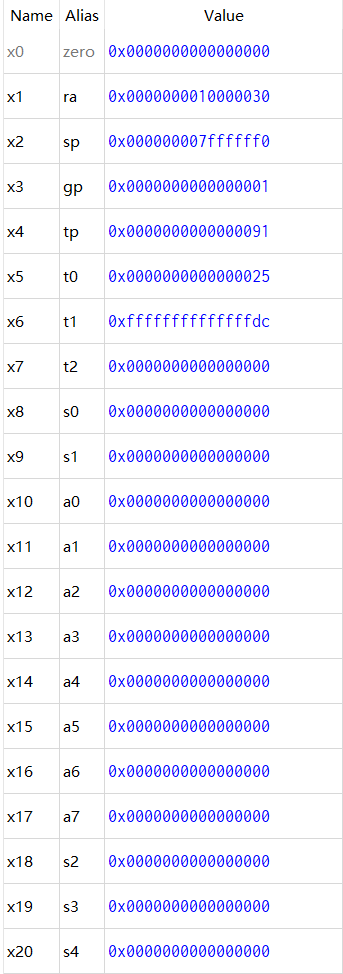
\includegraphics[scale=0.5]{fig4.png}
        \caption{任务二Ripes运行程序后各寄存器的值}
        \label{fig:lab2_ripes}
    \end{figure}
    
    
    之后,我们考虑将上述代码迁移到自己所设计的单周期CPU中。我们发现,在上述代码实现中涉及到\verb|bge|指令,而这一指令我们之前并没有进行译码。由此,我们需要对控制单元和ALU均作出修改。在本实验中,我们首先在ALU中添加信号\verb|positive|用以代表信号是否为正数,这一信号与\verb|z|信号用于表示信号是否为零的效果类似,其RISC-V实现也非常简单:
\begin{lstlisting}[language=verilog]
assign positive = (s[31] == 0); // positive means the MSB is 1
\end{lstlisting}

    之后,我们仿照\verb|beq|和\verb|bne|的译码模块,并根据标准RISC-V的语法设置函数的\verb|opcode|和\verb|func3|的值,并输出相应的控制信号。在本实验中,我们做出的修改可总结如下:\verb|pcsource|的修正,\verb|aluc|加入\verb|bge|指令,\verb|sext|加入\verb|bge|指令。

\begin{lstlisting}[language=verilog]
assign pcsource[1] = i_jalr | i_jal;
// pcsource[0] modified so that i_bge can jump when necessary (the result of sub is finite)
assign pcsource[0] = ( i_beq & z ) | (i_bne & ~z) | i_jal | (i_bge & positive) ;
\end{lstlisting}

    最后,在\verb|sc_computer|模块中修改端口的定义,并加入\verb|positive|信号便可以完成新指令的添加功能。我们将上述汇编语言加入程序的指令存储器中,并在CPU上执行仿真模拟,结果如图\ref{lab2_sim}所示。从中我们可以看出,程序正确地执行了新添加的分支指令,并得到了\verb|0x91|和\verb|0x01|这两个最大、最小值,并进一步地将其输出到对应的输出端口中。而执行的时钟周期数为\verb|0xfa|,代表\verb|CYC 250|,也即真实情况的\verb|125|个时钟周期,输出正确。

    \begin{figure}[htbp]
        \centering
        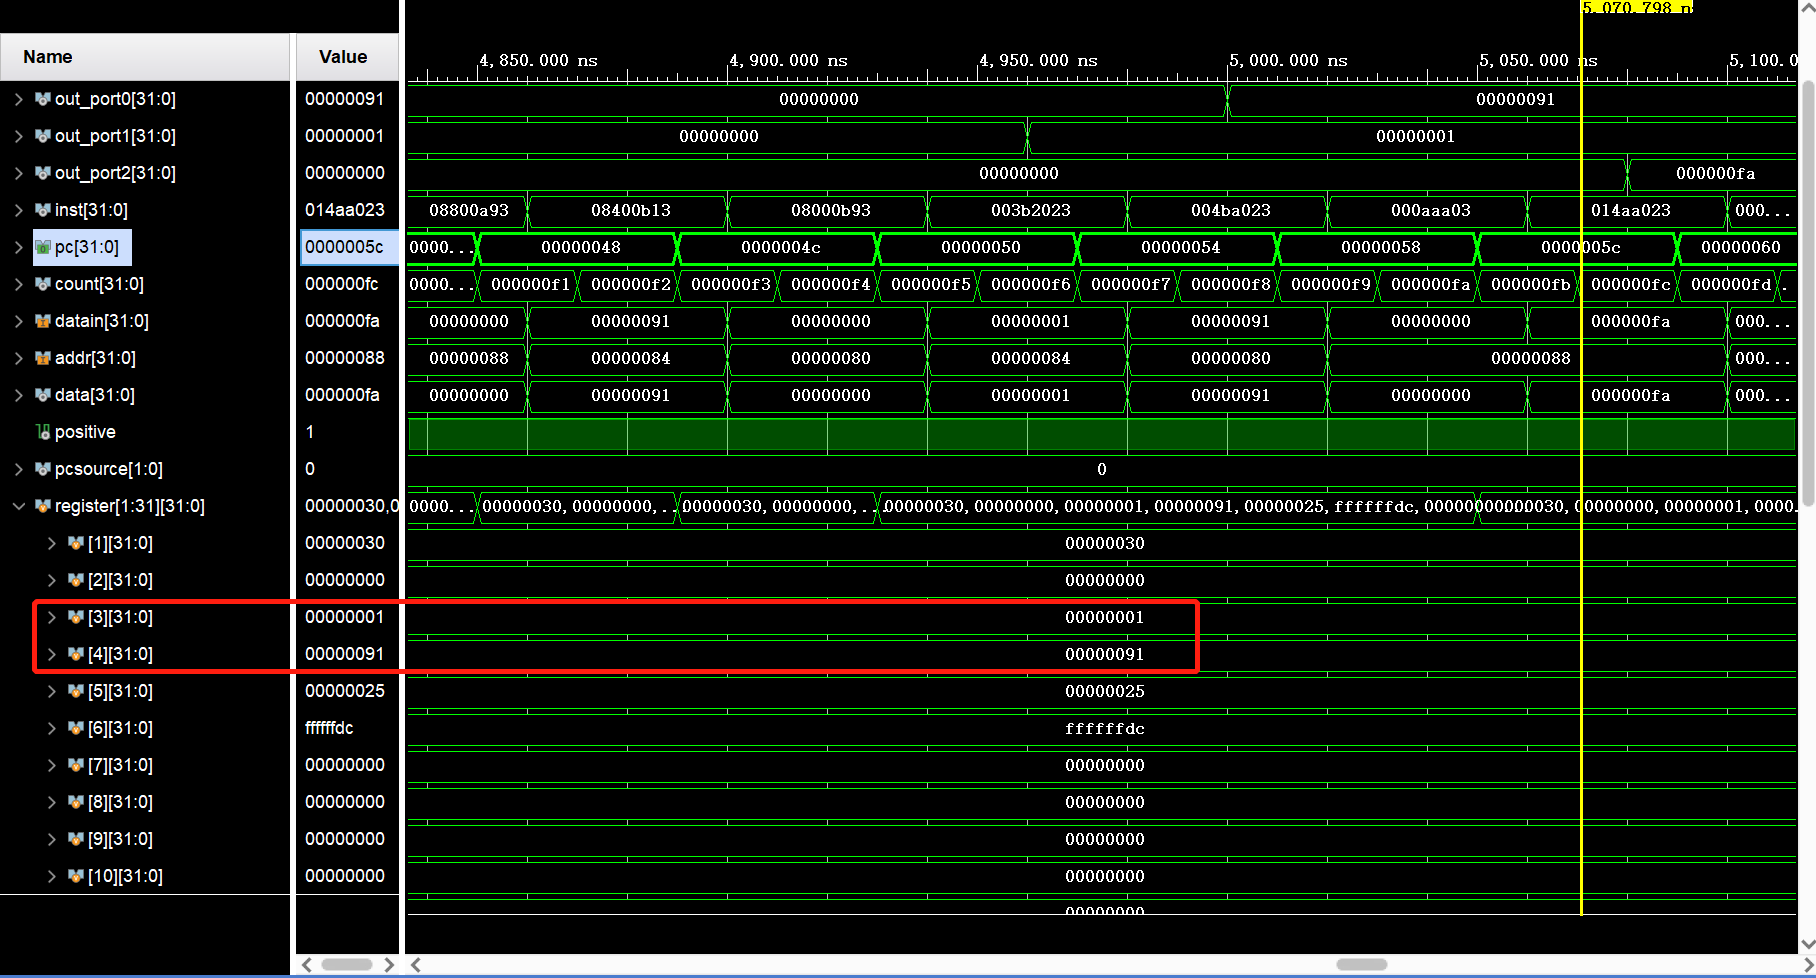
\includegraphics[scale=0.5]{fig5.png}
        \caption{实验二仿真结果}
        \label{fig:lab2_sim}
    \end{figure}

    在验证的最后,我们将程序烧录在FPGA板上来进行测试,结果如图\ref{fig:lab2_board}所示。最高两位为学号的后两位\verb|17|,之后四位分别为最大值和最小值对应的十进制数(\verb|145|和\verb|01|的后两位),而最后的两位则是时钟周期数的后两位\verb|50|。从中我们可以看出,我们设计的汇编程序和对CPU的相应修改能够达到预期的结果。

    \begin{figure}[htbp]
        \centering
        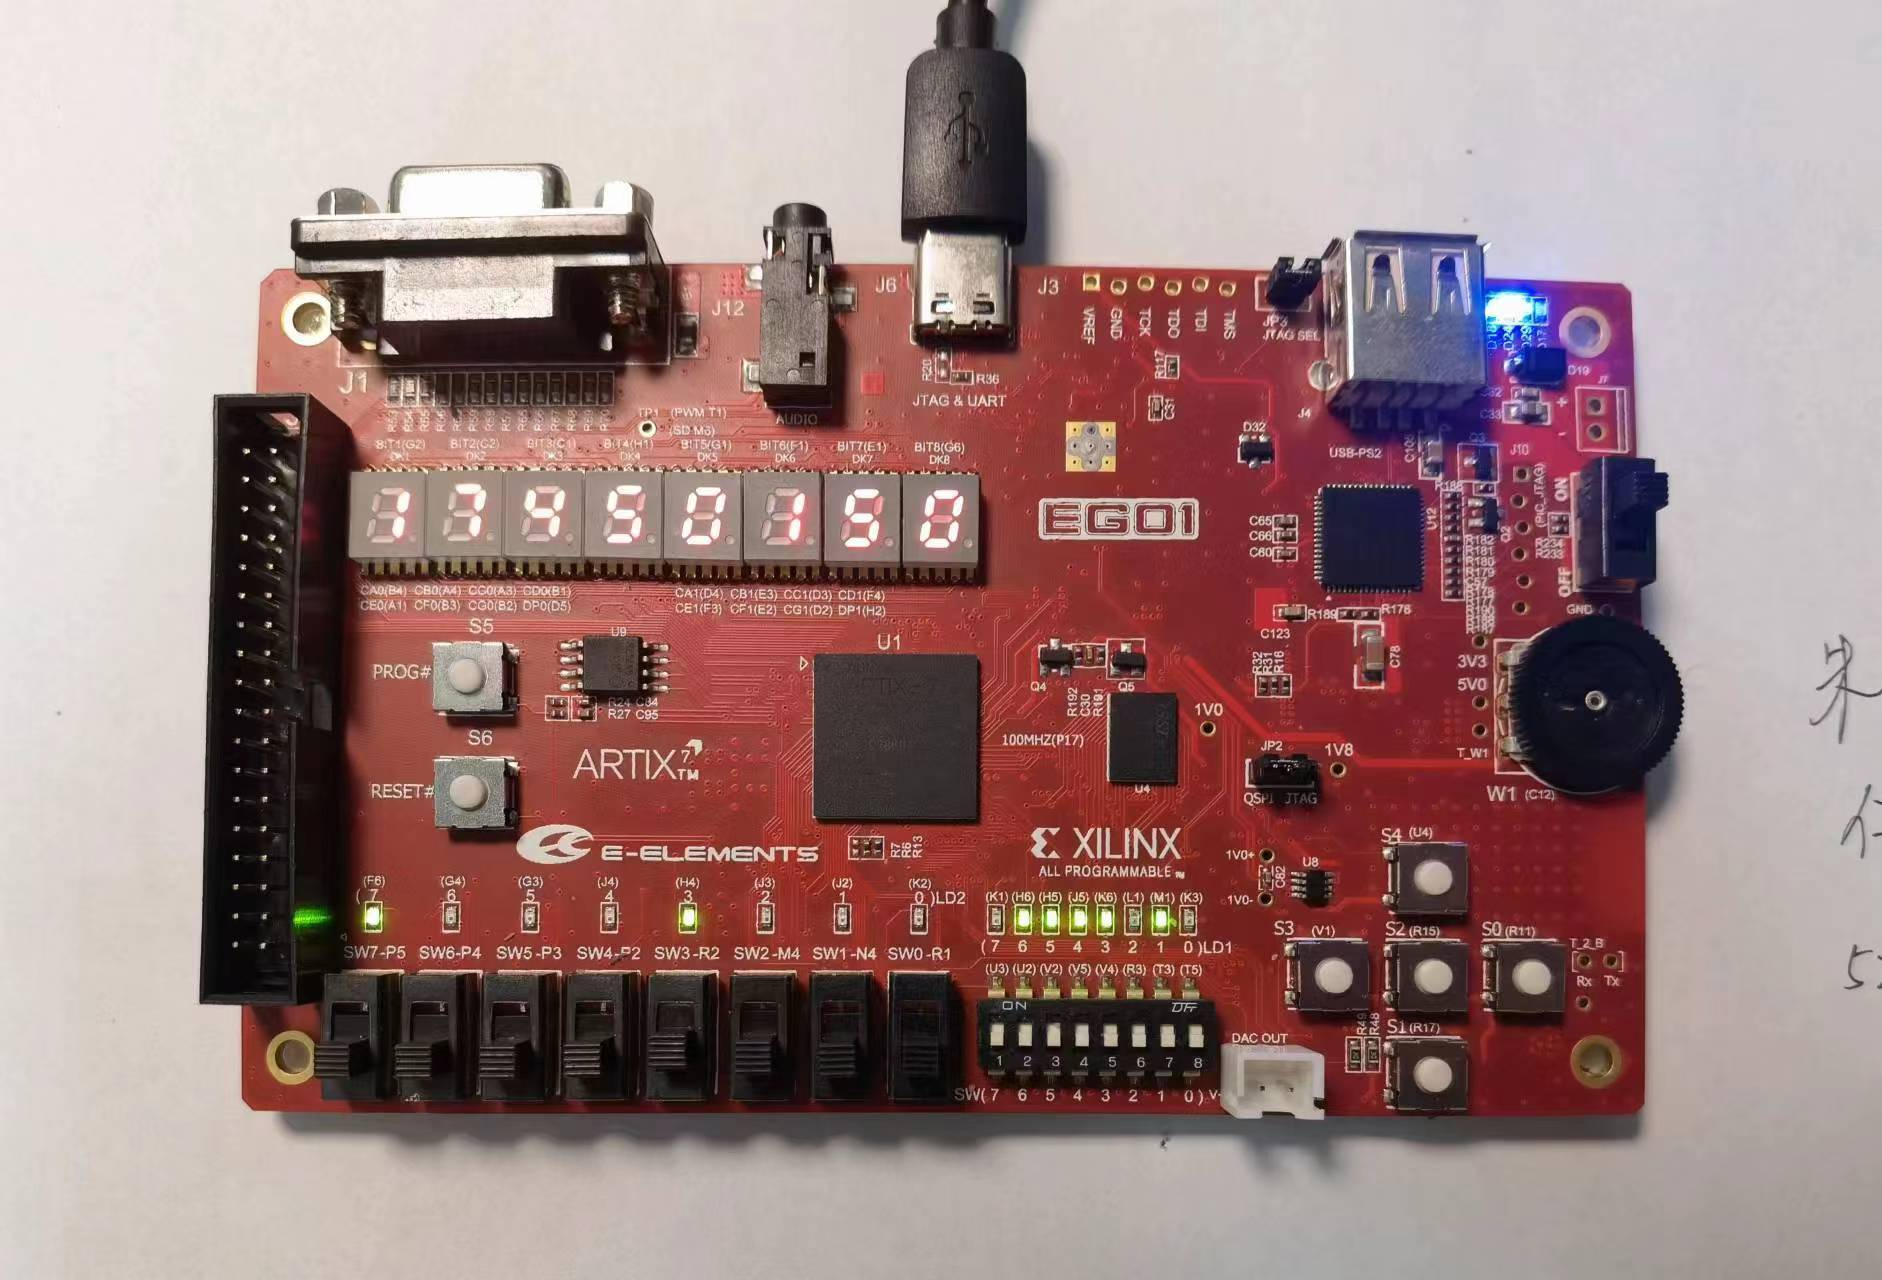
\includegraphics[scale=0.15]{fig6.jpg}
        \caption{实验二板级验证结果}
        \label{fig:lab2_board}
    \end{figure}

    \section{总结}

    作为ICE2603课程的实验大作业,我在实践的过程中能切实感受到对硬件操作能力的提升。从一开始对Verilog语言特性的完全不熟悉,到现在可以自己根据功能来设计一些简单的模块。从看实验指导书都费劲,到现在可以较为游刃有余地修改给定的模版。这一过程本身还是充满成就感的,从中也让自己对于CPU内部的指令译码、执行等过程有了较为深入的了解。希望本门课程中所积累的经验,能够为自己未来的发展打下更加坚实的基础。

\end{document}